%%%%%%%%%%%%%%%%%%%%%%%%%%%%%%%%%%%%%%%%%12pt: grandezza carattere
                                        %a4paper: formato a4
                                        %openright: apre i capitoli a destra
                                        %twoside: serve per fare un
                                        %   documento fronteretro
                                        %report: stile tesi (oppure book)
\documentclass[12pt,a4paper,openright,twoside]{report}
%
%%%%%%%%%%%%%%%%%%%%%%%%%%%%%%%%%%%%%%%%%libreria per scrivere in italiano
\usepackage[italian]{babel}
\usepackage{listings}
%
%%%%%%%%%%%%%%%%%%%%%%%%%%%%%%%%%%%%%%%%%libreria per accettare i caratteri
                                        %   digitati da tastiera come � �
                                        %   si pu� usare anche
                                        %   \usepackage[T1]{fontenc}
                                        %   per� con questa libreria
                                        %   il tempo di compilazione
                                        %   aumenta
\usepackage[latin1]{inputenc}
%
%%%%%%%%%%%%%%%%%%%%%%%%%%%%%%%%%%%%%%%%%libreria per impostare il documento
\usepackage{fancyhdr}
%
%%%%%%%%%%%%%%%%%%%%%%%%%%%%%%%%%%%%%%%%%libreria per avere l'indentazione
%%%%%%%%%%%%%%%%%%%%%%%%%%%%%%%%%%%%%%%%%   all'inizio dei capitoli, ...
\usepackage{indentfirst}
%
%%%%%%%%%libreria per mostrare le etichette
%\usepackage{showkeys}
%
%%%%%%%%%%%%%%%%%%%%%%%%%%%%%%%%%%%%%%%%%libreria per inserire grafici
\usepackage{graphicx}
\graphixpath{ ./images/ }
%
%%%%%%%%%%%%%%%%%%%%%%%%%%%%%%%%%%%%%%%%%libreria per utilizzare font
                                        %   particolari ad esempio
                                        %   \textsc{}
\usepackage{newlfont}
%
%%%%%%%%%%%%%%%%%%%%%%%%%%%%%%%%%%%%%%%%%librerie matematiche
\usepackage{amssymb}
\usepackage{amsmath}
\usepackage{latexsym}
\usepackage{amsthm}
%
\oddsidemargin=30pt \evensidemargin=20pt%impostano i margini
\hyphenation{sil-la-ba-zio-ne pa-ren-te-si}%serve per la sillabazione: tra parentesi
					   %vanno inserite come nell'esempio le parole
%					   %che latex non riesce a tagliare nel modo giusto andando a capo.

%
%%%%%%%%%%%%%%%%%%%%%%%%%%%%%%%%%%%%%%%%%comandi per l'impostazione
                                        %   della pagina, vedi il manuale
                                        %   della libreria fancyhdr
                                        %   per ulteriori delucidazioni
\pagestyle{fancy}\addtolength{\headwidth}{20pt}
\renewcommand{\chaptermark}[1]{\markboth{\thechapter.\ #1}{}}
\renewcommand{\sectionmark}[1]{\markright{\thesection \ #1}{}}
\rhead[\fancyplain{}{\bfseries\leftmark}]{\fancyplain{}{\bfseries\thepage}}
\cfoot{}
%%%%%%%%%%%%%%%%%%%%%%%%%%%%%%%%%%%%%%%%%
\linespread{1.3}                        %comando per impostare l'interlinea
%%%%%%%%%%%%%%%%%%%%%%%%%%%%%%%%%%%%%%%%%definisce nuovi comandi
%
\begin{document}
\begin{titlepage}                       %crea un ambiente libero da vincoli
                                        %   di margini e grandezza caratteri:
                                        %   si pu\`o modificare quello che si
                                        %   vuole, tanto fuori da questo
                                        %   ambiente tutto viene ristabilito
%
\thispagestyle{empty}                   %elimina il numero della pagina
\topmargin=6.5cm                        %imposta il margina superiore a 6.5cm
\raggedleft                             %incolonna la scrittura a destra
\large                                  %aumenta la grandezza del carattere
                                        %   a 14pt
\em                                     %emfatizza (corsivo) il carattere
Alla mia famiglia, \\
che mi ha sempre sostenuto \\
in ogni mia scelta.                      %\ldots lascia tre puntini
\newpage                                %va in una pagina nuova
%
%%%%%%%%%%%%%%%%%%%%%%%%%%%%%%%%%%%%%%%%
\clearpage{\pagestyle{empty}\cleardoublepage}%non numera l'ultima pagina sinistra
\end{titlepage}
\pagenumbering{roman}                   %serve per mettere i numeri romani
\chapter*{Introduzione}                 %crea l'introduzione (un capitolo
                                        %   non numerato)
%%%%%%%%%%%%%%%%%%%%%%%%%%%%%%%%%%%%%%%%%imposta l'intestazione di pagina
\rhead[\fancyplain{}{\bfseries
INTRODUZIONE}]{\fancyplain{}{\bfseries\thepage}}
\lhead[\fancyplain{}{\bfseries\thepage}]{\fancyplain{}{\bfseries
INTRODUZIONE}}
%%%%%%%%%%%%%%%%%%%%%%%%%%%%%%%%%%%%%%%%%aggiunge la voce Introduzione
                                        %   nell'indice
\addcontentsline{toc}{chapter}{Introduzione}
Questa \`e l'introduzione.
%%%%%%%%%%%%%%%%%%%%%%%%%%%%%%%%%%%%%%%%%non numera l'ultima pagina sinistra
\clearpage{\pagestyle{empty}\cleardoublepage}
\tableofcontents                        %crea l'indice
%%%%%%%%%%%%%%%%%%%%%%%%%%%%%%%%%%%%%%%%%imposta l'intestazione di pagina
\rhead[\fancyplain{}{\bfseries\leftmark}]{\fancyplain{}{\bfseries\thepage}}
\lhead[\fancyplain{}{\bfseries\thepage}]{\fancyplain{}{\bfseries
INDICE}}
%%%%%%%%%%%%%%%%%%%%%%%%%%%%%%%%%%%%%%%%%non numera l'ultima pagina sinistra
\clearpage{\pagestyle{empty}\cleardoublepage}
\listoffigures                          %crea l'elenco delle figure
%%%%%%%%%%%%%%%%%%%%%%%%%%%%%%%%%%%%%%%%%non numera l'ultima pagina sinistra
\clearpage{\pagestyle{empty}\cleardoublepage}
\listoftables                           %crea l'elenco delle tabelle
%%%%%%%%%%%%%%%%%%%%%%%%%%%%%%%%%%%%%%%%%non numera l'ultima pagina sinistra
\clearpage{\pagestyle{empty}\cleardoublepage}
\chapter{Lo stato dell'Arte}                %crea il capitolo
%%%%%%%%%%%%%%%%%%%%%%%%%%%%%%%%%%%%%%%%%imposta l'intestazione di pagina
\lhead[\fancyplain{}{\bfseries\thepage}]{\fancyplain{}{\bfseries\rightmark}}
\pagenumbering{arabic}                  %mette i numeri arabi
In questo capitolo si va ad illustrare lo stato dell'Arte delle tecnologie utilizzate.
Si illustreranno le principali qualit\`a degli Intrusion Detection Systems e le caratteristiche
principali che hanno portato durante i test alla scelta di un software rispetto che un altro.
Si passer\`a poi a presentare sFlow, illustrandone i benefici e le principali differenze
con NetFlow e di come esso viene attualmente utilizzato per affiancare un IDS.
Infine si dar\`a una breve presentazione dello stack ELK, (Elasticsearch-Logstash-Kibana)
e di come esso sia utilizzato nell'ambito della Network Security.
\section{Intrusion Detection System}                 %crea la sezione
Il panorama degli Intrusion Detection System (IDS) \`e al giorno d'oggi in continua evoluzione.
Tuttavia \`e possibile classificarli secondo due criteri principali che ne determinano il funzionamento:
\begin{itemize}
  \item Sistemi signature based
  \item Sistemi basati su anomaly detection
\end{itemize}

Un IDS signature based analizza i pacchetti passanti su una rete utilizzando un set di regole
appositamente scritte per rilevare un determinato tipo di attacco. Questo ci mette al riparo
da una grandissima quantit\`a di attacchi conosciuti e si \`e rilevato nel corso degli anni
un sistema efficiente e ampiamente utilizzato.

I secondi invece utilizzano tecniche di intelligenza artificiale per determinare se
un comportamento sia lecito oppure no basandosi su quello che \`e stato definito
in fase di installazione come uno "stato normale".

Sebbene nell'ultimo periodo l'intelligenza artificiale stia facendo la sua comparsa in ogni
ambito dell'informatica gli IDS signature based rappresentano tuttora un'importante
fetta (se non la maggioranza) degli IDS in uso nei pi\`u importanti data center del mondo
ed \`e per questo che vale la pena studiarli.


Tra i maggiori esponenti degli IDS attualmente utilizzati abbiamo:
\begin{itemize}
  \item Snort: Un IDS sviluppato a partire dagli anni '90, acquisito da Cisco nel 2013 e
  che \`e tuttora il pi\`u utilizzato in ambito enterprise.
  \item Suricata: Un IDS del nuovo millennio, sviluppato a partire dal 2009 da
  Open Information Security Foundation (OISF) e che vanta molteplici vantaggi sopra gli altri IDS.
\end{itemize}

In questo elaborato si \`e preferito utilizzare per motivi di performance e di implementazione,
Suricata. I dettagli di questa scelta saranno chiari pi\`u avanti quando saranno state
introdotte le principali caratteristiche di Suricata.

\subsection{Suricata, una breve introduzione}
Suricata \`e un IDS che fa uso di pattern matching per il riconoscimento di threat
capace di effettuare un'analisi molto approfondita. Il funzionamento del pattern matching pu\`o
essere riassunto dalla figura 1.1.
\begin{figure}
  \begin{center}                          %centra nel mezzo della pagina
    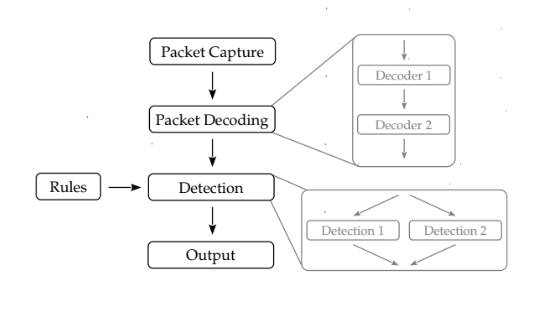
\includegraphics[width=90mm]{images/suricata-structure.png}
    \caption{Funzionamento del patter matching}
    \label{}
  \end{center}
\end{figure}
Mentre una tipica regola per il patter matching \`e fatta in questo modo:
\begin{verbatim}
  rule header    alert tcp any any -> 192.168.1.0/24 111
\end{verbatim}



E' stato dimostrato infatti (trovare il paper) che data la sua natura multi threaded
Suricata \`e di gran lunga pi\`u veloce di Snort, il quale invece \`e single thread.
La preferenza dell'uno rispetto all'altro non \`e tuttavia fondamentale dal punto di
vista dei risultati generati dai nostri test. Infatti Suricata utilizza lo stesso rule-set di
Snort.



\newpage

\section{Seconda Sezione}
Ora vediamo un elenco puntato:
\begin{itemize}                         %crea un elenco puntato
\item primo oggetto
\item secondo oggetto
\end{itemize}

\section{Altra Sezione}
Vediamo un elenco descrittivo:
\begin{description}                     %crea un elenco descrittivo
  \item[OGGETTO1] prima descrizione;
  \item[OGGETTO2] seconda descrizione;
  \item[OGGETTO3] terza descrizione.
\end{description}
%%%%%%%%%%%%%%%%%%%%%%%%%%%%%%%%%%%%%%%%%crea una sottosezione
\subsection{Altra SottoSezione}
%%%%%%%%%%%%%%%%%%%%%%%%%%%%%%%%%%%%%%%%%crea una sottosottosezione
\subsubsection{SottoSottoSezione}Questa sottosottosezione non viene
numerata, ma \`e solo scritta in grassetto.
\section{Altra Sezione}                 %crea una sottosezione
Vediamo la creazione di una tabella; la tabella \ref{tab:uno}
(richiamo il nome della tabella utilizzando la label che ho messo sotto):
la facciamo di tre righe e tre colonne, la prima colonna
``incolonnata'' a destra (r) e le altre centrate (c):\\
\begin{table}[h]                        %ambiente tabella
                                        %(serve per avere la legenda)
\begin{center}                          %centra nella pagina la tabella
\begin{tabular}{r|c|c}                  %tre colonne con righe verticali
                                        %   prodotte con |
\hline \hline                           %inserisce due righe orizzontali
$(1,1)$ & $(1,2)$ & $(1,3)$\\           %& separa le colonne e con
\hline                                  %inserisce una riga orizzontale
$(2,1)$ & $(2,2)$ & $(2,3)$\\           %  \\ va a capo
\hline                                  %inserisce una riga orizzontale
$(3,1)$ & $(3,2)$ & $(3,3)$\\
\hline \hline                           %inserisce due righe orizzontali
\end{tabular}
\caption[legenda elenco tabelle]{legenda tabella}\label{tab:uno}
\end{center}
\end{table}
\section{Altra Sezione}\label{sec:prova}%posso mettere le label anche
                                        %   alle section
\subsection{Listati dei programmi}
\subsubsection{Primo Listato}
\begin{verbatim}
        In questo ambiente     posso scrivere      come voglio,
lasciare gli spazi che voglio e non % commentare quando voglio
e ci sar� scritto tutto.
Quando lo uso � meglio che disattivi il Wrap del WinEdt
\end{verbatim}
%%%%%%%%%%%%%%%%%%%%%%%%%%%%%%%%%%%%%%%%%non numera l'ultima pagina sinistra
\clearpage{\pagestyle{empty}\cleardoublepage}
%%%%%%%%%%%%%%%%%%%%%%%%%%%%%%%%%%%%%%%%%per fare le conclusioni
\chapter*{Conclusioni}
%%%%%%%%%%%%%%%%%%%%%%%%%%%%%%%%%%%%%%%%%imposta l'intestazione di pagina
\rhead[\fancyplain{}{\bfseries
CONCLUSIONI}]{\fancyplain{}{\bfseries\thepage}}
\lhead[\fancyplain{}{\bfseries\thepage}]{\fancyplain{}{\bfseries
CONCLUSIONI}}
%%%%%%%%%%%%%%%%%%%%%%%%%%%%%%%%%%%%%%%%%aggiunge la voce Conclusioni
                                        %   nell'indice
\addcontentsline{toc}{chapter}{Conclusioni} Queste sono le
conclusioni.\\
In queste conclusioni voglio fare un riferimento alla
bibliografia: questo \`e il mio riferimento \cite{K3,K4}.
%%%%%%%%%%%%%%%%%%%%%%%%%%%%%%%%%%%%%%%%%imposta l'intestazione di pagina
\renewcommand{\chaptermark}[1]{\markright{\thechapter \ #1}{}}
\lhead[\fancyplain{}{\bfseries\thepage}]{\fancyplain{}{\bfseries\rightmark}}
\appendix                               %imposta le appendici
\chapter{Prima Appendice}               %crea l'appendice
In questa Appendice non si \`e utilizzato il comando:\\
%%%%%%%%%%%%%%%%%%%%%%%%%%%%%%%%%%%%%%%%%\verb"" � equivalente all'
                                        %   ambiente verbatim,
                                        %   ma si utilizza all'interno
                                        %   di un discorso.
\verb"\clearpage{\pagestyle{empty}\cleardoublepage}", ed infatti
l'ultima pagina 8 ha l'intestazione con il numero di pagina in
alto.
%%%%%%%%%%%%%%%%%%%%%%%%%%%%%%%%%%%%%%%%%imposta l'intestazione di pagina
\rhead[\fancyplain{}{\bfseries \thechapter \:Prima Appendice}]
{\fancyplain{}{\bfseries\thepage}}
\chapter{Seconda Appendice}             %crea l'appendice
%%%%%%%%%%%%%%%%%%%%%%%%%%%%%%%%%%%%%%%%%imposta l'intestazione di pagina
\rhead[\fancyplain{}{\bfseries \thechapter \:Seconda Appendice}]
{\fancyplain{}{\bfseries\thepage}}
\begin{thebibliography}{90}             %crea l'ambiente bibliografia
\rhead[\fancyplain{}{\bfseries \leftmark}]{\fancyplain{}{\bfseries
\thepage}}
%%%%%%%%%%%%%%%%%%%%%%%%%%%%%%%%%%%%%%%%%aggiunge la voce Bibliografia
                                        %   nell'indice
\addcontentsline{toc}{chapter}{Bibliografia}
%%%%%%%%%%%%%%%%%%%%%%%%%%%%%%%%%%%%%%%%%provare anche questo comando:
%%%%%%%%%%%\addcontentsline{toc}{chapter}{\numberline{}{Bibliografia}}
\bibitem{K1} Primo oggetto bibliografia.
\bibitem{K2} Secondo oggetto bibliografia.
\bibitem{K3} Terzo oggetto bibliografia.
\bibitem{K4} Quarto oggetto bibliografia.
\end{thebibliography}
%%%%%%%%%%%%%%%%%%%%%%%%%%%%%%%%%%%%%%%%%non numera l'ultima pagina sinistra
\clearpage{\pagestyle{empty}\cleardoublepage}
\chapter*{Ringraziamenti}
\thispagestyle{empty}
Qui possiamo ringraziare il mondo intero!!!!!!!!!!\\
Ovviamente solo se uno vuole, non \`e obbligatorio.
\end{document}
